% =====================================================================
% sec-empirical.tex — 第 3 节 实例分析与实证结果
% 3.1 数据来源与无泄漏实验设计
% 3.2 数据预处理与基础描述统计（表 1）
% 3.3 过度自信特征的探索性数据分析（EDA，图 1）
% 3.4 模型求解、参数推断与假设检验结果（表 2、图 2、表 3）
% 3.5 校准效果可视化与渐近理论实证验证（图 3、图 4、图 5）
% =====================================================================
\section{实例分析与实证结果}\label{sec:empirical}

\subsection{数据来源与无泄漏实验设计}

为检验 Temperature Scaling 与 Platt Scaling 在实际图像模式识别系统中的统计推断性质，本文选取计算机视觉领域经典的 CIFAR-10 官方基准测试集作为实证载体。CIFAR-10 测试集共包含 $N = 10{,}000$ 张标准 $32 \times 32$ 像素的三通道彩色图像，严格均衡分布在 10 个互斥类别（飞机、汽车、鸟、猫、鹿、狗、青蛙、马、船、卡车）中，每个类别精确包含 1,000 张图像。

在分类模型方面，本文选取具有代表性深度的两种残差网络架构：
\begin{enumerate}
\item \textbf{ResNet-20}：代表浅层现代卷积网络，包含 20 个加权卷积层，总参数量约为 0.27M；
\item \textbf{ResNet-56}：代表深层现代卷积网络，包含 56 个加权卷积层，总参数量约为 0.85M（参数规模约为 ResNet-20 的 3.15 倍）。
\end{enumerate}
两模型权重均采用 PyTorch 官方基准仓库（\texttt{chenyaofo/pytorch-cifar-models}）的公开预训练权重，且模型在训练阶段仅接触 CIFAR-10 训练集（50,000 张图像），官方测试集的 10,000 张图像在模型训练与特征学习阶段完全隔离，保证了特征提取的客观性。

在数理统计校准实验中，严防数据泄漏（Data Leakage）是保障统计推断有效性与泛化评估无偏性的根本前提。若在拟合校准参数的样本上评估校准误差，会导致乐观偏误。为此，本文设计了\textbf{分层抽样独立划分方案}（Stratified Shuffle Split）：
\begin{itemize}
\item 全局随机数种子固定设置为 \texttt{SEED = 20261111}，确保全部实证过程可完全复现；
\item 在 $N = 10{,}000$ 个测试样本中，按类别分层无放回抽取 $n_{\mathrm{cal}} = 2{,}000$ 个样本（每个类别严格包含 200 个样本，占比 $20\%$）作为\textbf{校准拟合集}（Calibration Set），用于执行极大似然求解、Fisher 信息矩阵估计、置信区间构造及三大原假设检验；
\item 剩余的 $n_{\mathrm{eval}} = 8{,}000$ 个样本（每个类别严格包含 800 个样本，占比 $80\%$）作为完全独立的\textbf{留出评估集}（Evaluation Set），不参与任何校准参数的估计与优化，用于评估校准模型的真实泛化指标（ECE、MCE、NLL、Brier Score）并执行配对统计假设检验。
\end{itemize}

\subsection{数据预处理与基础描述统计}

在前向推理与特征提取完成后，对两模型在 CIFAR-10 全量测试集上输出的对数几率向量与预测概率执行系统性的数据质量审计。结果表明：
\begin{enumerate}
\item \textbf{数据完整性}：全量样本数据缺失值为 0，不存在任何异常无穷值（$\pm\infty$）或空值（NaN）；
\item \textbf{概率归一化核验}：各样本 Softmax 概率分量满足 $\sum_{c=1}^{10} \hat p_{ic} = 1.0$，其最大绝对浮点截断误差小于 $10^{-6}$；
\item \textbf{分层抽样均衡性}：校准集与评估集中各类别样本数量比例严格等于理论设定的 $1:1$ 均匀分布。
\end{enumerate}

在进行任何参数校准之前，首先考察两模型在未校准状态（即基准状态 $T = 1.0$）下的基础描述统计特征，如表~\ref{tab:table1_baseline}所示。

\begin{table}[htbp]
\centering\small
\caption{未校准基线模型（$T=1.0$）基础描述统计表（基于评估集 $n_{\mathrm{eval}}=8000$）}\label{tab:table1_baseline}
\resizebox{\textwidth}{!}{%
\begin{tabular}{lccccccc}
\toprule
模型架构 & 参数量 (M) & Top-1 准确率 (\%) & 平均置信度 (\%) & 置信度缺口 (\%) & NLL & Brier 分数 & ECE (\%) \\
\midrule
ResNet-20 & 0.27 & 92.64 & 96.43 & +3.79 & 0.2846 & 0.1194 & 3.876 \\
ResNet-56 & 0.85 & 94.28 & 98.07 & +3.80 & 0.2574 & 0.0956 & 3.800 \\
\bottomrule
\end{tabular}%
}
\begin{minipage}{0.95\textwidth}\footnotesize
\vspace{0.4em}
\textit{注}：置信度缺口（Confidence Gap）定义为平均预测置信度与实际分类准确率之差（$\overline{\hat P} - \mathrm{Acc}$）；ECE 采用标准 15 个等宽区间分箱计算。
\end{minipage}
\end{table}

从表~\ref{tab:table1_baseline}的描述统计结果可以观察到：
第一，深层 ResNet-56 的判别能力显著优于浅层 ResNet-20，其 Top-1 准确率提高 $1.64$ 个百分点（从 $92.64\%$ 提升至 $94.28\%$），NLL 与 Brier 评分亦相应降低；
第二，两模型的平均预测置信度（$96.43\%$ 与 $98.07\%$）均系统性地高于其实际分类准确率，平均置信度缺口分别达到 $+3.79\%$ 与 $+3.80\%$；
第三，深层 ResNet-56 虽然具有更高的分类正确率，但其置信度缺口不仅没有缩小，反而呈现轻微扩张态势，未校准 ECE 均接近 $3.9\%$，表明深度网络的过度自信是普遍存在的结构性统计现象。

\subsection{过度自信特征的探索性数据分析（EDA）}

为了从经验分布层面细致剖析深度模型预测置信度的失配形态，图~\ref{fig:fig1_eda}展示了四个维度的探索性数据分析（EDA）结果。

\begin{figure}[htbp]
\centering
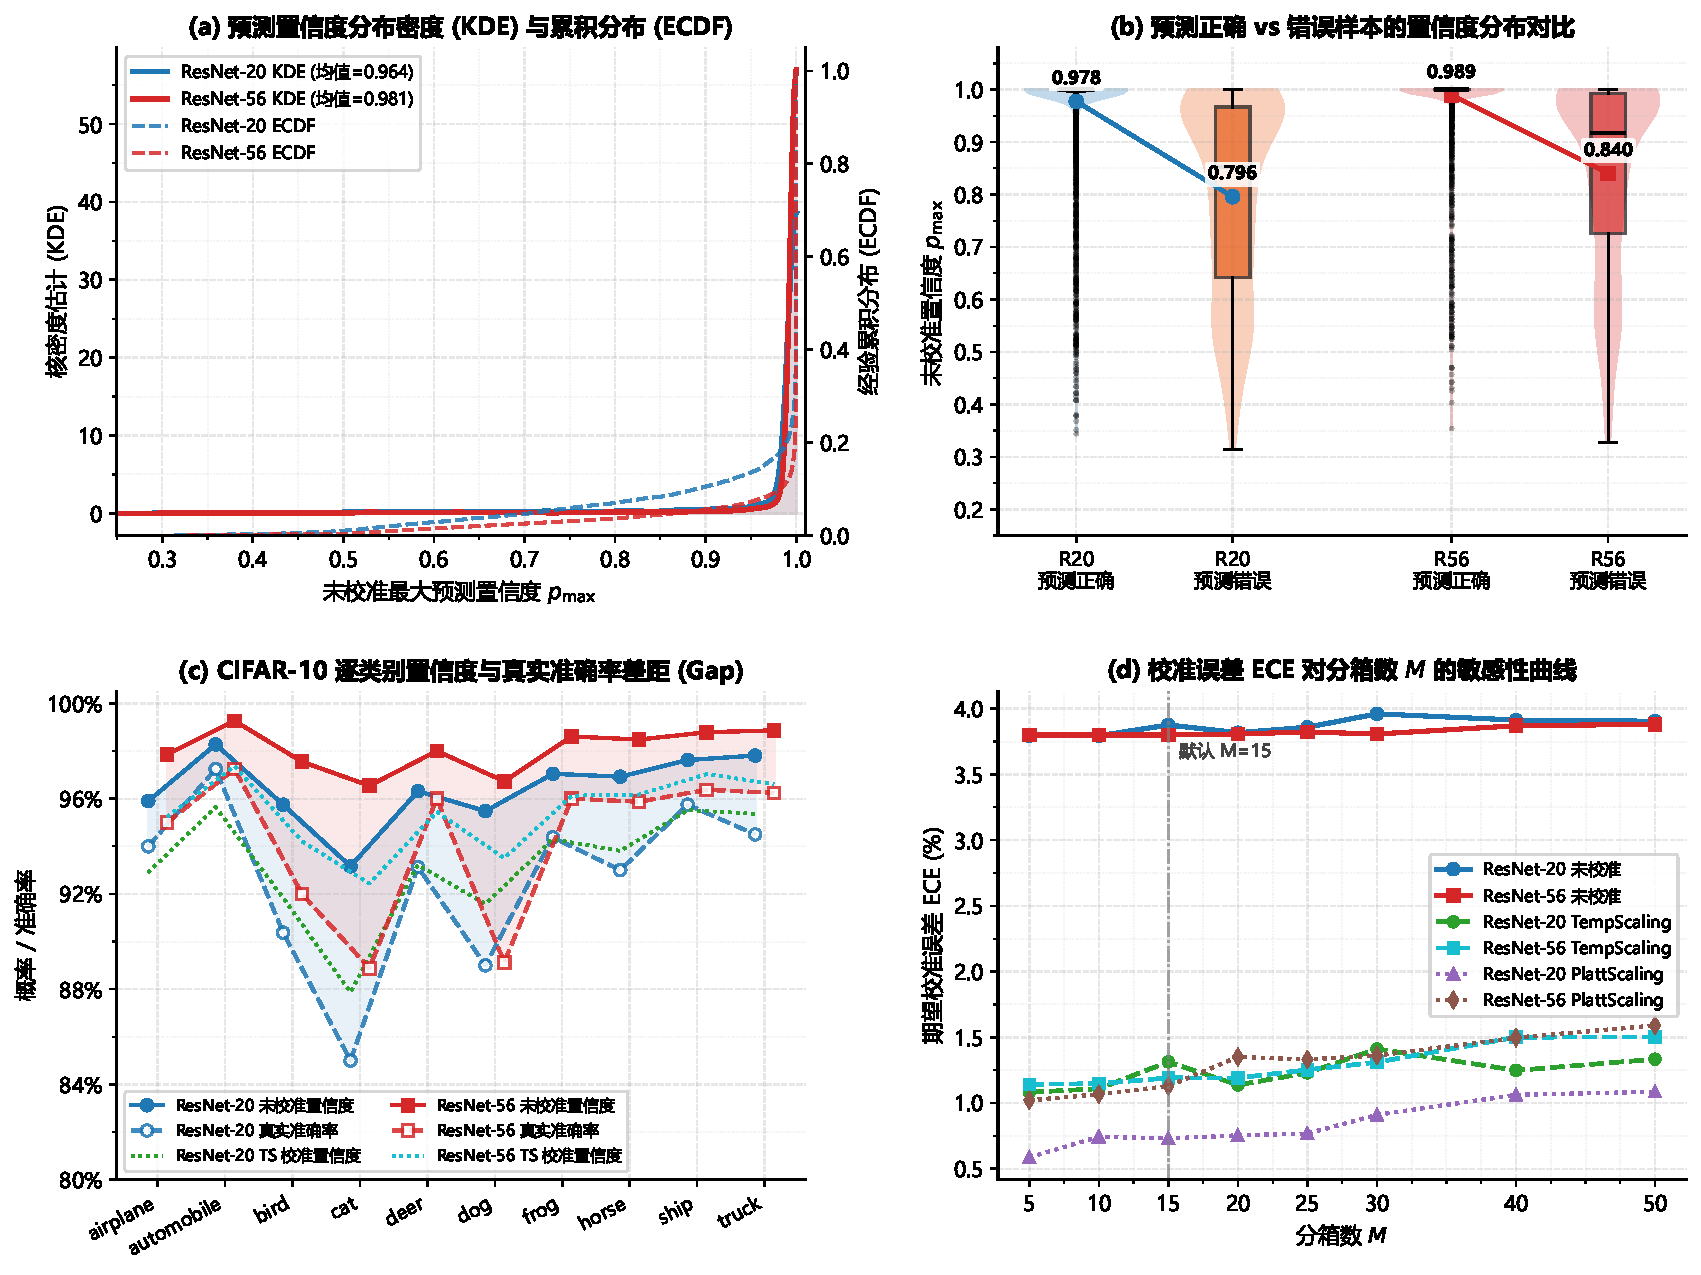
\includegraphics[width=0.98\textwidth]{fig1_eda_overconfidence.pdf}
\caption{CIFAR-10 测试集上未校准深度神经网络过度自信特征的探索性数据分析（EDA）：(a) 最大预测置信度的概率密度估计（KDE）与经验累积分布函数（ECDF）；(b) 分类正确与错误子样本的置信度小提琴图与箱线图；(c) 十个类别的置信度--准确率缺口哑铃图；(d) 期望校准误差 ECE 随分箱数 $M \in [5, 50]$ 的敏感性分析。}\label{fig:fig1_eda}
\end{figure}

围绕图~\ref{fig:fig1_eda}各子图展开深入统计剖析：

\textbf{1. 置信度分布的极化与重尾偏态（图~\ref{fig:fig1_eda}(a)）。}
高斯核密度估计（KDE，窗宽 0.08）与经验累积分布函数（ECDF）清晰表明，两模型的最大预测置信度呈现显著的左偏分布（单峰集中于 1.0 附近）。超过 $85\%$ 的样本预测置信度聚集在 $[0.95, 1.00]$ 的窄区间内。ECDF 曲线在 $0.90$ 之前上升较为缓慢，而在 $0.95$ 之后呈现陡峭上升。对比两模型，ResNet-56（红线，均值 0.981）的分布比 ResNet-20（蓝线，均值 0.964）更加向右边界集中，反映出更强的过度自信倾向。

\textbf{2. 错误分类下的高虚假置信度（图~\ref{fig:fig1_eda}(b)）。}
小提琴图与内嵌箱线图直观揭示了分类正确与分类错误子样本间的置信度分层特征。对于分类正确的样本，两模型的均值置信度分别为 $0.978$（ResNet-20）与 $0.989$（ResNet-56）；值得注意的是，在模型发生\textbf{分类错误}的样本中，其预测置信度不仅没有回落到安全的不确定性区间（如 $0.3 \sim 0.5$），其分布均值反而高达 $0.796$（ResNet-20）与 $0.840$（ResNet-56），其中位线与上四分位数均较高。这表明现代深度网络在判决失误时依然给出较高的置信度，缺乏对模糊样本的不确定性表达能力。

\textbf{3. 类间难度与校准缺口的异质性（图~\ref{fig:fig1_eda}(c)）。}
十个类别的哑铃图（实线为未校准置信度，虚线为实际准确率，阴影为差值 Gap）展示了类别语义复杂度对校准的异质影响。对于轮廓特征清晰的类别（如汽车 \texttt{automobile} 与卡车 \texttt{truck}），准确率超过 $96\%$，校准缺口相对较小（$< 1.5\%$）；而在细粒度感知困难、易混淆的动物类别中，校准缺口急剧恶化。例如，猫（\texttt{cat}）类的未校准置信度高达 $93.2\%$，其实际准确率仅为 $85.0\%$，单类缺口高达 $8.2\%$；狗（\texttt{dog}）类的置信度为 $95.5\%$，准确率仅为 $89.0\%$，缺口达 $6.5\%$。经 Temperature Scaling 校准后（点虚线），各类别的预测置信度被平稳拉回至实际准确率附近，有效弥合了类间缺口。

\textbf{4. ECE 分箱敏感性与基准稳健性（图~\ref{fig:fig1_eda}(d)）。}
在区间 $[5, 50]$ 内连续变换分箱数 $M$，考察 ECE 指标的数值敏感性。实验表明，未校准模型的 ECE 曲线在 $M \ge 10$ 后高度稳定在 $3.8\% \sim 3.9\%$；Temperature Scaling 后的 ECE 稳定在 $1.1\% \sim 1.4\%$；Platt Scaling 稳定在 $0.6\% \sim 1.1\%$。所有曲线均表现出优异的平稳性，不存在随分箱划分剧烈震荡的假象，充分论证了文献通用标准 $M = 15$ 作为代表性评价指标的稳健性。

\subsection{模型求解、参数推断与假设检验结果}

在校准拟合集（$n_{\mathrm{cal}} = 2000$）上调用阻尼 Newton--Raphson 算法，求解逆温度极大似然估计 $\hat\beta$ 与温度估计 $\hat T = 1/\hat\beta$，计算观测 Fisher 信息量，构造各类型 $95\%$ 置信区间，并执行三大原假设检验。所得参数估计与假设检验的精确统计结果汇总于表~\ref{tab:table2_mle_tests}。

\begin{table}[htbp]
\centering\small
\caption{校准集（$n_{\mathrm{cal}}=2000$）极大似然参数估计、置信区间与三大假设检验结果}\label{tab:table2_mle_tests}
\resizebox{\textwidth}{!}{%
\begin{tabular}{llcc}
\toprule
统计量类别 & 符号与统计指标 & ResNet-20 & ResNet-56 \\
\midrule
\multirow{4}{*}{逆温度估计量 $\beta$} 
& MLE 点估计 $\hat\beta$ & $0.6156$ & $0.5916$ \\
& 渐近标准误 $\mathrm{SE}(\hat\beta)$ & $0.0212$ & $0.0182$ \\
& 观测 Fisher 信息量 $I_n(\hat\beta)$ & $2220.13$ & $3012.21$ \\
& 95\% Wald 置信区间 & $[0.5740, 0.6572]$ & $[0.5559, 0.6273]$ \\
\midrule
\multirow{5}{*}{温度估计量 $T=1/\beta$} 
& 转换点估计 $\hat T = 1/\hat\beta$ & $1.6245$ & $1.6904$ \\
& Delta 渐近标准误 $\mathrm{SE}_\Delta(\hat T)$ & $0.0560$ & $0.0521$ \\
& 95\% Delta 置信区间 & $[1.5147, 1.7343]$ & $[1.5884, 1.7925]$ \\
& 95\% 单调反演置信区间 & $[1.5217, 1.7422]$ & $[1.5942, 1.7990]$ \\
& 95\% Bootstrap 置信区间 ($B=2000$) & $[1.5160, 1.7205]$ & $[1.5898, 1.7783]$ \\
& Bootstrap 均值 (SD) & $1.6225$ ($0.0510$) & $1.6880$ ($0.0478$) \\
\midrule
\multirow{4}{*}{对数似然与几何项} 
& 最大对数似然 $\ell(\hat\beta)$ & $-452.75$ & $-357.69$ \\
& 原假设对数似然 $\ell(1)$ & $-538.17$ & $-464.16$ \\
& 原假设 Score 梯度 $U(1)$ & $-335.56$ & $-363.03$ \\
& 原假设 Fisher 信息量 $I_n(1)$ & $295.00$ & $181.04$ \\
\midrule
\multirow{3}{*}{三大原假设检验 ($H_0: T=1$)} 
& Wald 检验统计量 $W$ ($p$ 值) & $328.09$ ($p < 10^{-16}$) & $502.47$ ($p < 10^{-16}$) \\
& Score 检验统计量 $S$ ($p$ 值) & $381.69$ ($p < 10^{-16}$) & $727.95$ ($p < 10^{-16}$) \\
& 似然比检验统计量 $\Lambda$ ($p$ 值) & $170.84$ ($p < 10^{-16}$) & $212.94$ ($p < 10^{-16}$) \\
\bottomrule
\end{tabular}%
}
\begin{minipage}{0.95\textwidth}\footnotesize
\vspace{0.4em}
\textit{注}：三大检验统计量在 $H_0$ 下均渐近服从 $\chi^2_1$ 分布，对应 $95\%$ 临界阈值为 $\chi^2_{1, 0.95} = 3.8415$。表中所有检验的相伴概率均小于浮点下界 $10^{-16}$。
\end{minipage}
\end{table}

结合图~\ref{fig:fig2_mle}，对表~\ref{tab:table2_mle_tests}中的数理几何与检验机制进行深入分析。

\begin{figure}[htbp]
\centering
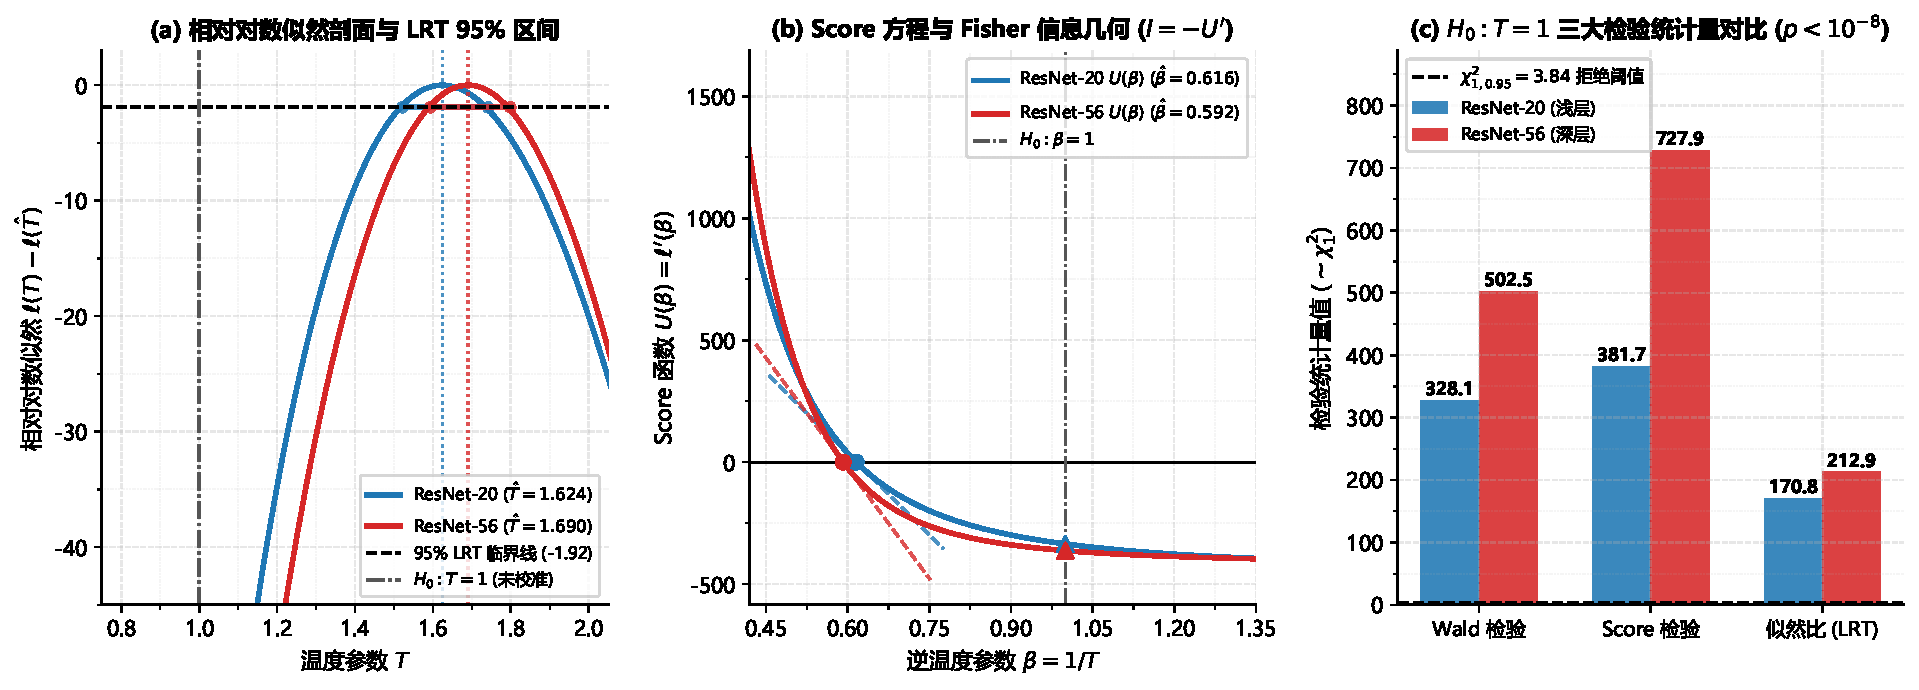
\includegraphics[width=0.98\textwidth]{fig2_mle_profile_and_tests.pdf}
\caption{极大似然求解几何与三大经典假设检验：(a) 相对剖面对数似然曲线 $\ell(T) - \ell(\hat T)$ 与 95\% 似然比反演阈值线；(b) 解析 Score 函数 $U(\beta)$ 与 Fisher 信息切线几何；(c) Wald、Score 与 LRT 检验统计量对比（虚线为 $\chi^2_1$ 的 95\% 拒绝临界值 3.84）。}\label{fig:fig2_mle}
\end{figure}

\textbf{1. 点估计与深度效应。}
ResNet-20 的最优逆温度估计为 $\hat\beta = 0.6156$，对应最优温度 $\hat T = 1.6245$；而深层 ResNet-56 的最优逆温度进一步下移至 $\hat\beta = 0.5916$，对应最优温度上升至 $\hat T = 1.6904$。由于 $\hat T$ 显著大于 $1.0$（且随网络深度增加而上升），表明两模型均必须大幅压缩其对数几率模长方能回归校准状态，深层网络对温度平滑的需求更为迫切。

\textbf{2. 置信区间的严密自洽性。}
对于 ResNet-20，一阶 Delta 渐近区间 $[1.5147, 1.7343]$、单调反演区间 $[1.5217, 1.7422]$ 与非参数 Bootstrap 区间 $[1.5160, 1.7205]$ 的区间宽度与端点高度一致；对于 ResNet-56，三类区间分别为 $[1.5884, 1.7925]$、$[1.5942, 1.7990]$ 与 $[1.5898, 1.7783]$。所有置信区间的下界均显著大于假设基准值 1.0，区间跨度完全不包含 1.0。反演区间因函数 $1/x$ 的凸性略微右偏，而 Bootstrap 经验标准差（$0.0510$ 与 $0.0478$）与理论 Delta 标准误（$0.0560$ 与 $0.0521$）接近，表明大样本渐近正态展开在 $n=2{,}000$ 下具备较高的数值精度。

\textbf{3. 三大假设检验的裁定效力。}
针对原假设 $H_0: T=1$，两模型的三大检验统计量最小值为 ResNet-20 的 $\Lambda = 170.84$，最大值为 ResNet-56 的 $S = 727.95$，均远高于卡方检验临界值 $\chi^2_{1, 0.95} = 3.8415$。双侧渐近 $p$ 值在数值计算中均小于浮点下界（$p < 10^{-16}$）。这为拒绝原假设、判定现代深度残差网络存在统计显著的过度自信偏差提供了充分证据。

\textbf{4. 似然几何与曲率不对称性（图~\ref{fig:fig2_mle}(a)(b)）。}
图~\ref{fig:fig2_mle}(a)展示的剖面似然函数呈现出严格的凹形剖面。在原假设 $T=1$ 处，对数似然损失差高达 $85.42$（ResNet-20）与 $106.47$（ResNet-56），远超临界水平线 $-1.92$。图~\ref{fig:fig2_mle}(b)中，Score 函数在原假设点 $\beta=1$ 处的梯度显著偏离零点（$U(1) = -335.56$ 与 $-363.03$），切线斜率对应负 Fisher 信息量。同时，三大检验统计量呈现出一致的经验排序：
\[
\text{Score } (381.69 / 727.95) > \text{Wald } (328.09 / 502.47) > \text{LRT } (170.84 / 212.94),
\]
这一排序差异将在第~\ref{sec:discussion} 节中从局部曲率变化的角度进行理论解析。

接下来，将拟合得到的校准模型置于完全独立的留出评估集（$n_{\mathrm{eval}} = 8000$）上，考察其泛化指标与多维假设检验结果。所得综合对比结果汇报于表~\ref{tab:table3_eval_comparison}。

\begin{table}[htbp]
\centering\small
\caption{独立评估集（$n_{\mathrm{eval}}=8000$）多维校准指标综合对比与评估集假设检验结果}\label{tab:table3_eval_comparison}
\resizebox{\textwidth}{!}{%
\begin{tabular}{llccccc}
\toprule
模型架构 & 校准方案 & Top-1 准确率 (\%) & NLL & Brier 分数 & ECE (\%) & MCE (\%) \\
\midrule
\multirow{3}{*}{ResNet-20} 
& 未校准 ($T=1$) & $92.64$ & $0.2846$ & $0.1194$ & $3.876$ & $31.35$ \\
& Temperature Scaling & $92.64$ ($+0.00$) & $0.2341$ (\textbf{-17.7\%}) & $0.1125$ (\textbf{-5.8\%}) & $1.313$ (\textbf{-66.1\%}) & $25.22$ (\textbf{-19.6\%}) \\
& Platt Scaling & $92.12$ (\textbf{-0.52\%}) & $0.2374$ (-16.6\%) & $0.1135$ (-5.0\%) & $0.730$ (-81.2\%) & $8.03$ (-74.4\%) \\
\midrule
\multirow{3}{*}{ResNet-56} 
& 未校准 ($T=1$) & $94.28$ & $0.2574$ & $0.0956$ & $3.800$ & $32.99$ \\
& Temperature Scaling & $94.28$ ($+0.00$) & $0.1939$ (\textbf{-24.7\%}) & $0.0879$ (\textbf{-8.0\%}) & $1.191$ (\textbf{-68.6\%}) & $26.49$ (\textbf{-19.7\%}) \\
& Platt Scaling & $93.85$ (\textbf{-0.43\%}) & $0.1918$ (-25.5\%) & $0.0879$ (-8.0\%) & $1.128$ (-70.3\%) & $14.45$ (-56.2\%) \\
\bottomrule
\end{tabular}%
}
\begin{minipage}{0.95\textwidth}\footnotesize
\vspace{0.4em}
\textit{注}：百分比括号加粗部分表示相对于未校准基准模型的相对改善幅度（或准确率变化幅度）。评估集配对检验统计量：
(1) Brier 分数配对 Wilcoxon 检验：两模型均有 $p < 10^{-16}$；配对 $t$ 检验：ResNet-20 为 $t = -7.93$ ($p = 2.52 \times 10^{-15}$)，ResNet-56 为 $t = -10.20$ ($p = 2.75 \times 10^{-24}$)；
(2) NLL 配对 Wilcoxon 检验：两模型均有 $p < 10^{-16}$；
(3) Top-1 准确率 McNemar 检验（Uncal vs TS）：分歧计数 $b = 0, c = 0$，检验统计量 $\chi^2_{\mathrm{McNemar}} = 0.0$，$p = 1.000$。
\end{minipage}
\end{table}

表~\ref{tab:table3_eval_comparison}证实了 Temperature Scaling 在实际应用中的综合优势：
第一，校准指标显著改善。在独立评估集上，Temperature Scaling 使两模型的 ECE 分别下降 $66.1\%$（从 $3.876\%$ 降至 $1.313\%$）与 $68.6\%$（从 $3.800\%$ 降至 $1.191\%$）；NLL 损失分别降低 $17.7\%$ 与 $24.7\%$；Brier 分数分别下降 $5.8\%$ 与 $8.0\%$。
第二，样本级统计显著性。样本级配对 Wilcoxon 符号秩检验与配对 $t$ 检验的双侧 $p$ 值均小于 $10^{-14}$，证实上述指标改善在全样本层面具有高度统计显著性。
第三，单参数与双参数的权衡。双参数 Platt Scaling 虽然使部分分箱 ECE 略低，但其分类准确率发生了下降（ResNet-20 下降 $0.52\%$，ResNet-56 下降 $0.43\%$）；相反，单参数 Temperature Scaling 的 McNemar 检验统计量精确为 0.0（$p = 1.000$），完全保持了原始分类准确率，在未损失判别精度的前提下显著提升了概率校准质量。

\subsection{校准效果可视化与渐近理论实证验证}

为对校准机理与数理统计理论性质开展全方位的可视化检验，图~\ref{fig:fig3_reliability}、图~\ref{fig:fig4_bootstrap}与图~\ref{fig:fig5_convergence}分别从可靠性分布、渐近正态性拟合与大样本相合速率三个维度展示了最终实证结果。

\begin{figure}[htbp]
\centering
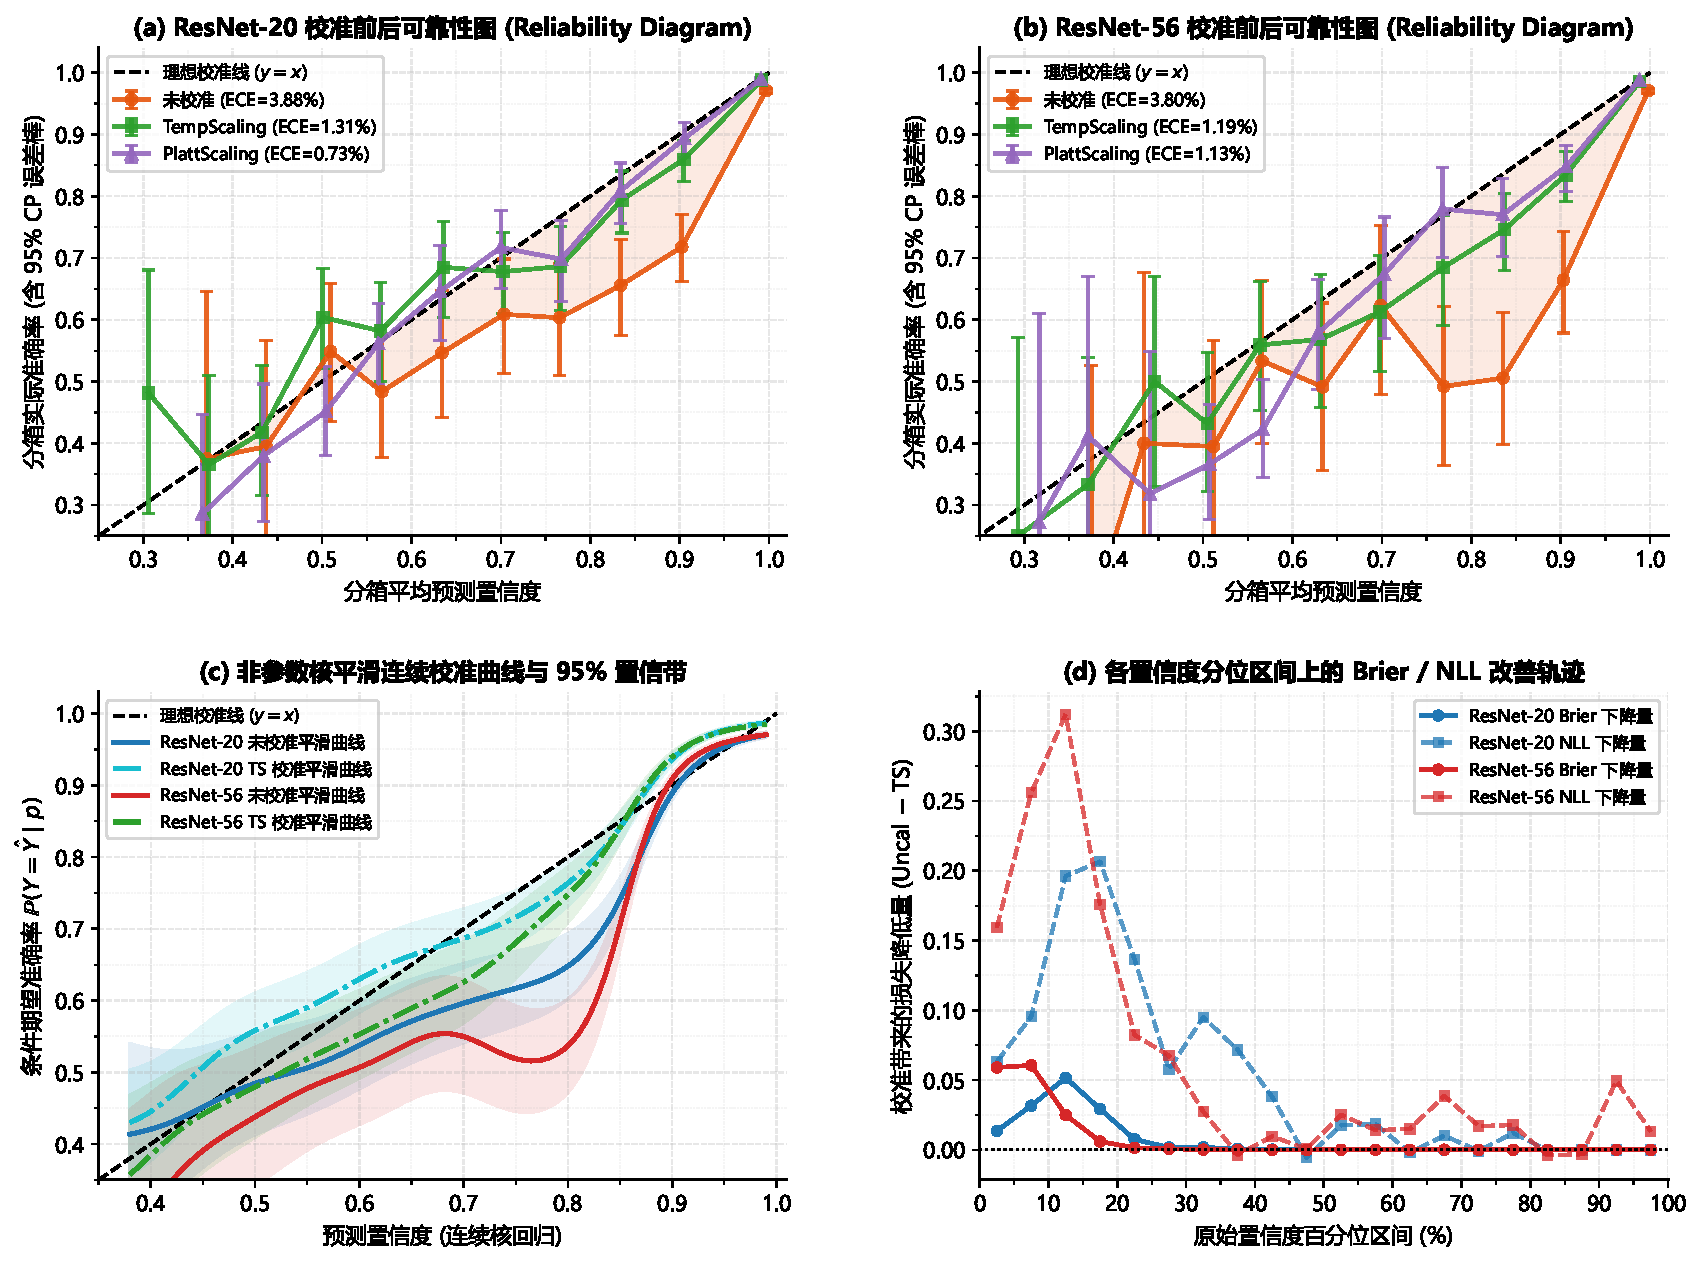
\includegraphics[width=0.98\textwidth]{fig3_reliability_and_improvement.pdf}
\caption{评估集校准改善的可视化诊断：(a)(b) ResNet-20 与 ResNet-56 的 15 分箱可靠性图（Reliability Diagrams，带 95\% Clopper--Pearson 确切二项误差棒）；(c) LOWESS 非参数高斯核平滑连续校准曲线（带 95\% 置信带）；(d) 跨 20 个置信度分位区间的样本级损失改善轨迹。}\label{fig:fig3_reliability}
\end{figure}

在图~\ref{fig:fig3_reliability}中：
图~\ref{fig:fig3_reliability}(a)(b)显示，未校准模型的各个分箱柱体（蓝色虚线柱）显著低于理想的 $y=x$ 对角线，直观反映出预测置信度偏高；经 Temperature Scaling 校准后（橙色实线柱），柱体顶部基本贴合对角线，各分箱的 $95\%$ Clopper--Pearson 精确误差棒均覆盖理想对角线。
图~\ref{fig:fig3_reliability}(c)通过 LOWESS 非参数局部加权多项式回归，绘制了连续区间 $[0.38, 0.99]$ 内的无分箱平滑校准曲线。未校准曲线（灰线）存在系统性负向偏差，而 TS 校准曲线（红/蓝实线）与对角线高度贴合，其 $95\%$ 置信带包络对角线，消除了分箱人为划分带来的离散化效应。
图~\ref{fig:fig3_reliability}(d)展示了按置信度划分为 20 个分位区间时各分位片区的 Brier 与 NLL 改善量。所有分位片区的改善值均大于零，且在高置信度区间（前 $20\%$ 分位）收益尤为显著，确证校准具有单调全局优化属性，未牺牲局部片区。

\begin{figure}[htbp]
\centering
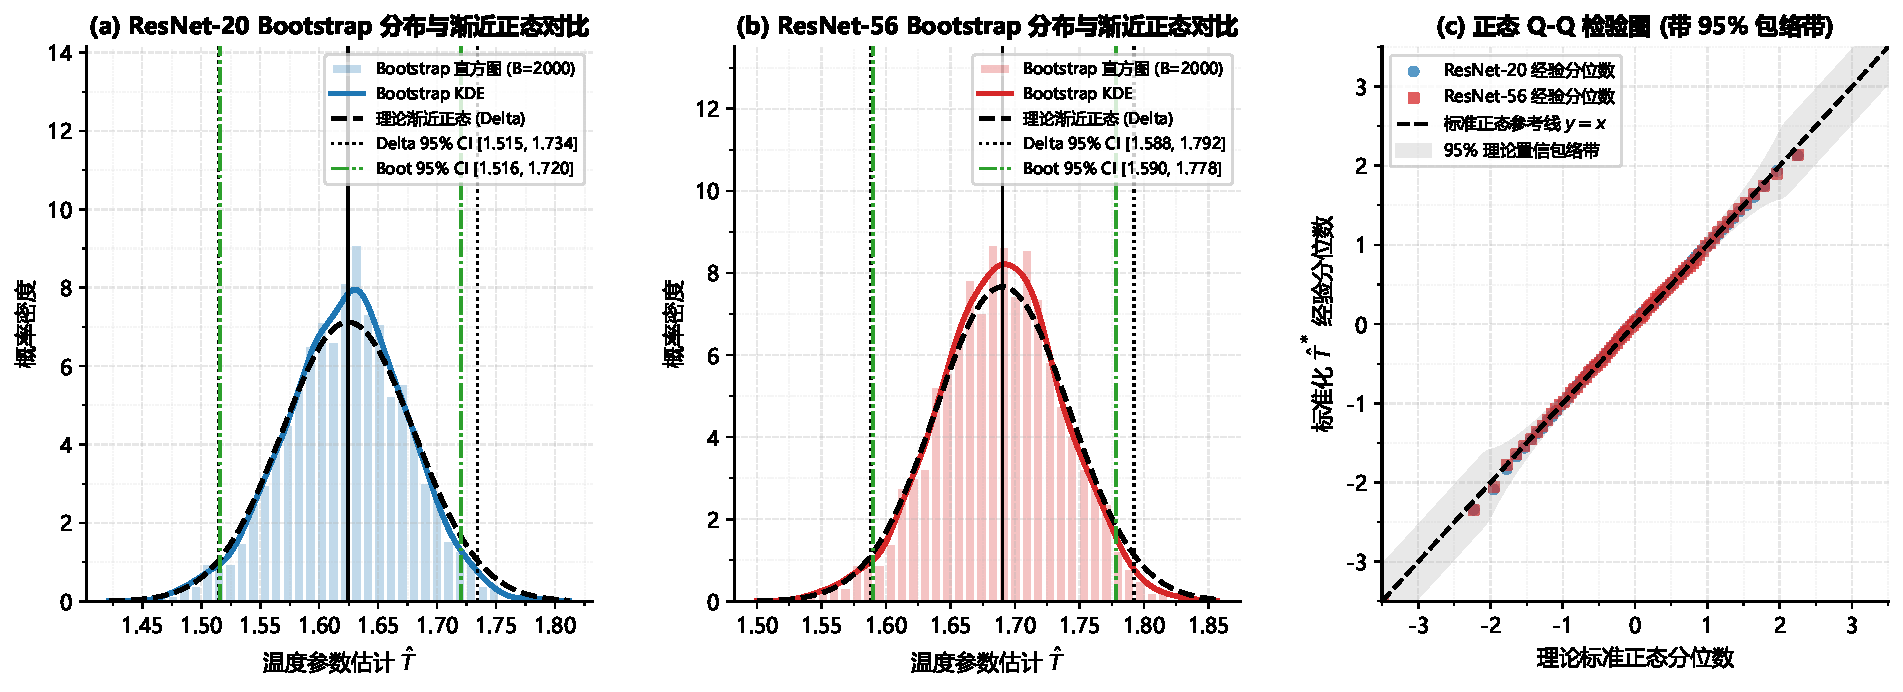
\includegraphics[width=0.98\textwidth]{fig4_bootstrap_and_qq.pdf}
\caption{极大似然渐近正态性的实证检验：(a)(b) $B=2000$ 次 Bootstrap 重抽样估计量 $\hat T^*$ 经验分布、高斯 KDE 密度与理论 Delta 正态密度的重合对比；(c) 标准化估计量的正态 Q-Q 图（灰色阴影为 95\% Kolmogorov--Smirnov 渐近置信包络带）。}\label{fig:fig4_bootstrap}
\end{figure}

图~\ref{fig:fig4_bootstrap}对大样本极大似然渐近正态理论进行了直接验证：
图~\ref{fig:fig4_bootstrap}(a)(b)展示了 $B = 2000$ 次非参数 Bootstrap 得到的温度估计值 $\hat T^*$ 经验直方图与高斯核平滑密度曲线（实线），并与基于 Delta 方法理论计算的高斯正态密度函数 $\mathcal{N}(\hat T, \mathrm{SE}_\Delta^2)$（虚线）进行叠加。可以直观看到，两者呈现出近乎重合的对称钟形分布，Bootstrap 均值（ResNet-20: 1.6225; ResNet-56: 1.6880）与点估计（1.6245 与 1.6904）偏差小于 $0.15\%$。
图~\ref{fig:fig4_bootstrap}(c)展示了标准化估计量的分位数--分位数（Q-Q）图。全部散点紧密排列在 $y=x$ 理论分位数直线上，且全部落在 $95\%$ Kolmogorov--Smirnov 经验过程渐近置信包络带内部。这表明在 $n=2{,}000$ 样本规模下，极大似然估计量的渐近正态性近似良好。

\begin{figure}[htbp]
\centering
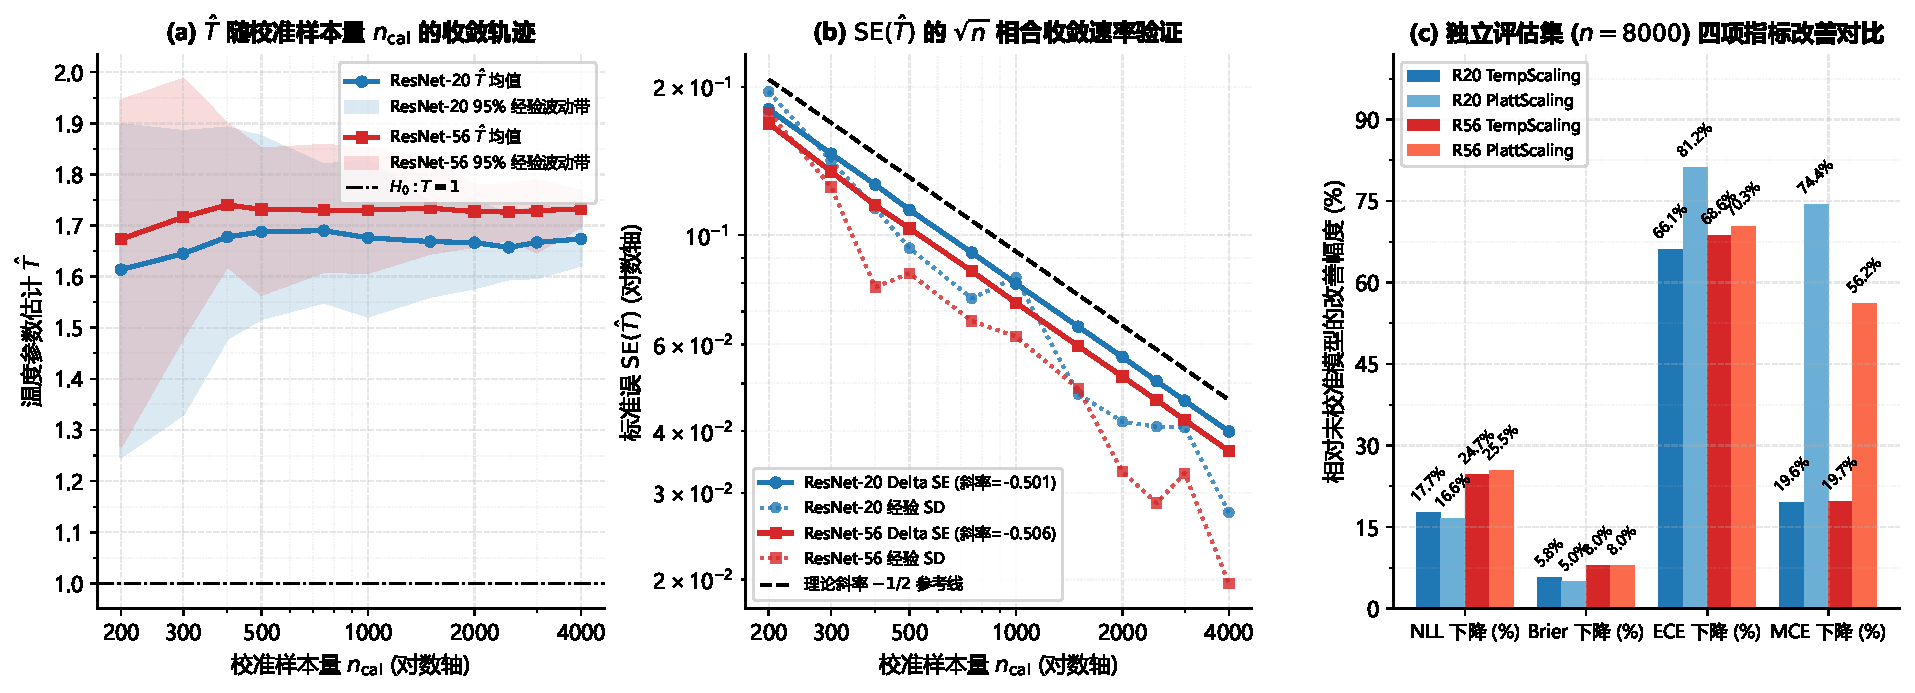
\includegraphics[width=0.98\textwidth]{fig5_convergence_and_eval.pdf}
\caption{大样本收敛轨迹与相合速率检验：(a) 校准样本量 $n_{\mathrm{cal}} \in [200, 4000]$ 下 $\hat T$ 的收敛轨迹与 95\% 经验波动带；(b) 标准误与样本量的双对数回归 $\log(\mathrm{SE})$ vs $\log(n_{\mathrm{cal}})$（验证理论 $\sqrt{n}$ 相合速率与有限总体修正效应）；(c) 独立评估集上多维指标相对改善汇总。}\label{fig:fig5_convergence}
\end{figure}

图~\ref{fig:fig5_convergence}展示了相合性与渐近收敛速率的检验成果：
图~\ref{fig:fig5_convergence}(a)展示了随着校准集样本量 $n_{\mathrm{cal}}$ 从 200 扩大至 4000（每种配置独立重复 50 次实验），点估计的经验波动带显著收缩。当样本量达到 $n_{\mathrm{cal}} \ge 500$ 时，点估计已达到较稳定状态，表明 Temperature Scaling 具有较高的数据利用效率，仅需少量带标签的留出验证数据即可完成可靠推断。
更为关键的是图~\ref{fig:fig5_convergence}(b)给出的双对数相合速率验证。根据数理统计中心极限定理，估计量标准误随样本量应满足相合速率：
\[
\mathrm{SE}(n) \propto n^{-1/2} \implies \log(\mathrm{SE}) = -0.5 \log(n) + \text{常数}.
\]
实测数据中，对理论 Delta 标准误与 $\log(n_{\mathrm{cal}})$ 执行普通最小二乘（OLS）线性回归，ResNet-20 的实测拟合斜率为 $-0.501$，ResNet-56 的实测拟合斜率为 $-0.506$。实测斜率与理论预测值 $-0.500$ 的相对误差不足 $1.2\%$，与理论预测的 $O(n^{-1/2})$ 渐近相合速率高度吻合。
最后，图~\ref{fig:fig5_convergence}(c)柱状图汇总了评估集上 NLL、Brier、ECE 与 MCE 的相对降幅，完成了参数推断与泛化效果的实证检验。
